\chapter{The Enigma}

\begin{chapquote}{Gordon Welchman, \textit{The Hut Six Story Page 52}}
  The Engima, though simple in principle and primitive in many ways,
  presented the cryptanalyst with a dazzling number of possibilities.
\end{chapquote}

The Engima machine was used extensivley by the Germans to encipher
communications prior to and throughout World War II. German
strategems like the \emph{blitzkrieg} required quick radio
communcation, so to ensure that the allied powers did not intercept
signals, they encoded all radio signals using the Enigma machine.
Breaking the Enigma would allow the allied powers to freely intercept
all naval, airforce, and military command -- offering them time to
counter, defend, and retaliate appropriately. Thus, while millions
participated in a war of arms and power, a select group of academics
at Bletchley park engaged in a battle of minds to crack a puzzle
whose solution could save millions of lives.

\section{The Machine}
Throughout this paper, the model \texttt{I} Enigma is chosen to
represent our canonical machine as these were the most common version
used during World War II with over 20000 being produced. Further, it
was used by both the \emph{Heer} (Army), \emph{Luftwaffe} (Air
Force), and the \emph{Kriegsmarine} (Navy) making this a prime target
for attack by cryptanalysts. Many models existed each with varying
layouts, keyspaces, and use-cases; however, the central ideas that
are discussed in this paper can generally be adapted to work on other models.
\\\\At its most basic function, the Enigma (once set up) is a
keyboard, whose letters, when depressed, illuminate bulbs of a
corresponding keyboard layout. The operator presses keys of the
desired plaintext and copies the output of the illuminated bulbs to
get the enciphered text. The actual mechanism of this encipherment
requires several mechanical components in a complex arrangement
\subsubsection{The Plugboard}
\text{}\\
\begin{center}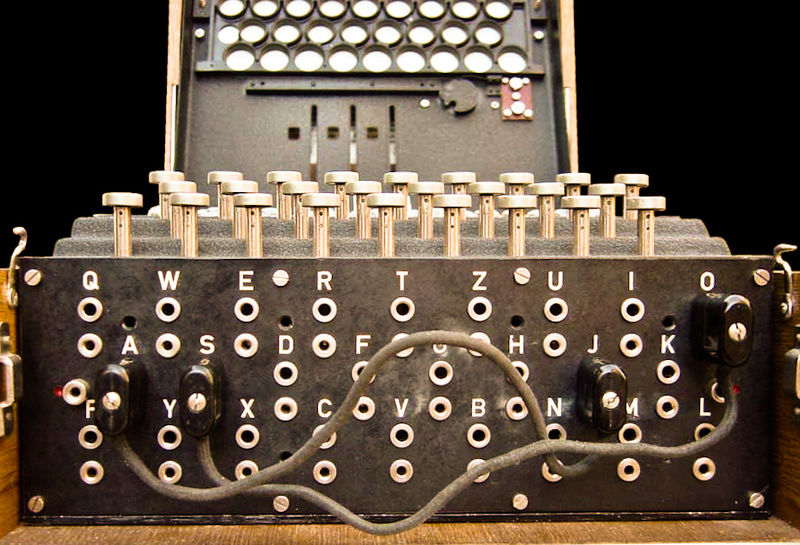
\includegraphics{plugboard.jpg}
\end{center}
Upon a key press, the electrical current corresponding to this letter
is sent to a mechanism known as the plugboard. From an operator's
perspective, the plugboard was a series of ports, one for each
letter, along with 10 cables which could connect these ports. When
two letters are connected via a cable (e.g. A and Z), the plugboard
will send current corresponding to a letter to the opposite letter
(e.g. A goes to Z and vice versa). If no cable is plugged in to a
letter (e.g. D has no cable), then the plugboard simply will return a
current corresponding to this same letter (e.g. D). Assuming all 10
cables are used this means that the plugboard can be represented as a
permutation on 26 letters with a cycle type of $2^{10}1^6$. One such
permutation could be
\begin{center}
  (\texttt{HR})(\texttt{AT})(\texttt{IW})(\texttt{SK})(\texttt{UY})(\texttt{DF})(\texttt{GV})(\texttt{LJ})(\texttt{BQ})(\texttt{MX})(\texttt{C})(\texttt{E})(\texttt{N})(\texttt{O})(\texttt{P})(\texttt{Z})
\end{center}
In general we will denote the permutation corresponding to a plugboard as $P$.

\subsubsection{The Rotors}

\subsubsection{The Reflector}

\section{The Enigma Protocol}
Before describing the internal mechanics of the Enigma, we will first
view the machine as an operator might.
%% https://bletchleypark.org.uk/our-story/enigmas-of-bletchley-park/%%
%% https://www.cryptomuseum.com/crypto/enigma/i/index.htm%%
%% https://www.cryptomuseum.com/crypto/enigma/files/schluessel_m.pdf%^
\\\\Suppose Alice and Bob are two radio operators (between September
1938 and May 1940) who want to communicate securely. Each are
supplied an Enigma machine along with a machine key
(\emph{maschinenschlussel}). THe machine key

Further, each have a copy of the ``\emph{General Regulations for the
Enigma}'' -- a book entailing all the protocols necessary for Alice
and Bob to communicate securely. According to this guide ``all secret
communcations are to be enciphered on the Engima'', in order to do
this, the following guides are necessary external to the machine itself
\begin{itemize}
  \item The general daily key (\emph{Tagesschluessel Allgemein})
  \item The K-Book (\emph{K-Buch})
\end{itemize}

% \\\begin{figure}[h]
%   \begin{center}
%     \resizebox{0.98\textwidth}{!}{
% \begin{tabular}{|c|c|c|c|c|}
% \hline
% \textbf{\emph{\texttt{Datum}}} &
% \textbf{\emph{\texttt{Walzenlage}}} &
% \textbf{\emph{\texttt{Ringstellung}}} &
% \textbf{\emph{\texttt{Steckerverbindungen}}} &
% \textbf{\emph{\texttt{Grundstellung}}} \\
% \hline
% \texttt{31.} & \texttt{IV II I} & \texttt{F T R} & \texttt{HR AT IW
% SK UY DF GV LJ BQ MX}   & \texttt{sfy azy zkq bqi} \\
% \texttt{30.} & \texttt{III V II} & \texttt{Y V P} & \texttt{OR KI
% JV }   & \texttt{iuy swz omo myj} \\
% \texttt{29.} & \texttt{V IV I} & \texttt{O H R} & \texttt{WJ VD PO
% MQ FX ZR NE LG UO BK}   & \texttt{rui kao fqi rwu} \\
%   $\vdots$ & $\vdots$ & $\vdots$ & $\vdots$ & $\vdots$ \\

% \hline
% \end{tabular}}
% \end{center}
%   \caption{Example Engima Key Sheet (September 1938)}
%   \label{fig:enigma_key_sheet}
% \end{figure}
%% https://www.researchgate.net/figure/Enigma-key-book-Photo-from-authentic-German-codebook-From-before-September-1938-as-it_fig2_339932418
% %%

% \\\begin{figure}[h]
%   \begin{center}
%     \resizebox{0.98\textwidth}{!}{
% \begin{tabular}{|c|c|c|c|c|}
% \hline
% \textbf{\emph{\texttt{Datum}}} &
% \textbf{\emph{\texttt{Walzenlage}}} &
% \textbf{\emph{\texttt{Ringstellung}}} &
% \textbf{\emph{\texttt{Steckerverbindungen}}} &
% \textbf{\emph{\texttt{Kenngruppen}}} \\
% \hline
% \texttt{31.} & \texttt{V II IV} & \texttt{17 09 02} & \texttt{KT AJ
% IV UR NY HZ GD XF PB CQ}   & \texttt{sfy azy zkq bqi} \\
% \texttt{30.} & \texttt{I III V} & \texttt{22 12 10} & \texttt{UE PL
% AY TB ZH WM OJ DC KN SI}   & \texttt{iuy swz omo myj} \\
% \texttt{29.} & \texttt{V IV II} & \texttt{04 01 25} & \texttt{WJ VD
% PO MQ FX ZR NE LG UO BK}   & \texttt{rui kao fqi rwu} \\
% \texttt{28.} & \texttt{II III IV}  & \texttt{05 03 12} & \texttt{HR
% TJ LD IO CN GX QK PZ WS AF}   & \texttt{ioy kjv yko fpz} \\
% $\vdots$ & $\vdots$ & $\vdots$ & $\vdots$ & $\vdots$ \\
% \hline
% \end{tabular}}
% \end{center}
%   \caption{Mock Enigma Key Sheet for April 1943.}
%   \label{fig:enigma_key_sheet}
% \end{figure}
